
\documentclass[fleqn,10pt]{article} % Document font size and equations flushed left


\usepackage{hyperref} % Required for hyperlinks
\usepackage{graphicx}
\usepackage[english]{babel}
\usepackage{caption}
\DeclareGraphicsExtensions{.pdf,.png,.jpg}


\begin{document}

\title{Article Title} % Article title

\author{Tom Newport} % Authors
\maketitle


\begin{abstract}
There's nothing here yet
\end{abstract}

\maketitle % Print the title and abstract box

\tableofcontents % Print the contents section

\thispagestyle{empty} % Removes page numbering from the first page

%----------------------------------------------------------------------------------------
%	ARTICLE CONTENTS
%----------------------------------------------------------------------------------------
% Total word count should be approx. 4500 words

% Add command to format binomial species name:
\newcommand{\bn}
[1]{\textit{#1}}

% Add shortcut for P. falciparum
\newcommand{\pf}
{\bn{P. falciparum }}

% Add semantic strong (replaces bold)
\newcommand{\str}
[1]{\textbf{#1}}

\section{Introduction} 

%% TN Introduce Plasmodium falciparum, establish that it lives inside red blood cells
The apicomplexan parasite \bn{Plasmodium falciparum} is the most virulent causative agent of malaria, and responsible for over 600,000 deaths annually \cite{WorldHealthOrganisation2013}. Along with other members of the \bn{Plasmodium} family, \pf has a complex lifecycle, moving between several different tissues in both mammalian and arthropod hosts. Symptomatic disease in humans occurs when \pf undergoes rounds of asexual reproduction inside human red blood cells (RBCs) \cite{Chen2000}.

%% TN Introduce RBC intracellular environment, benefits and challenges
In some respects, the intracellular environment of a red blood cell is an ideal location for parasite proliferation. The cells' lack of an MHC (Major Histocompatibility Complex) system, which would otherwise be used to identify intracellular pathogens to the host immune system, renders parasites immunologically invisible \cite{Kirchgatter2005}, whilst the vascular system allows the parasite to travel throughout the body. The highly specialised nature of RBCs, however, means that the intracellular environment also presents significant challenges to parasite survival.

%% TN Introduce challenges to pf survival
Mature red blood cells lack protein production and export machinery, and are a nutritionally poor environment, with a proteome dominated by haemoglobin, which typically accounts for around 98\% of the protein content of the cell \cite{DAlessandro2010}. \pf is able to digest RBC proteins, however haemoglobin lacks several amino acids required for protein production. Red blood cells are also  subject to regular 'quality control' in the spleen, where damaged or infected cells are killed and recycled \cite{Elsworth2014}.

%% TN Introduce exportome
In order to survive and proliferate inside RBCs, \pf exports a range of proteins which radically transform the red blood cell, collectively termed the \str{exportome}. Many of these proteins are involved in setting up a parasite-derived protein export system, capable of directing exported \pf proteins to sites both inside and outside the RBC. \pf resides inside a parasitophorous vacuole, and exports proteins via structures termed Maurer's Clefts \cite{Marti2013}, which bear some similarity to golgi apparatus \cite{Mundwiler-Pachlatko2013}.

%% TN Split paragraph
In order to avoid detection in the spleen, many exported proteins are associated with the formation of knobs, specialised structures which form at the RBC membrane and promote cytoadherence to epithelial cells, platelets and other red blood cells \cite{Kraemer2006}. Severe forms of malaria, including cerebral malaria, are believed to be caused by sequestration of infected red blood cells in deep tissues, as well as overinduction of inflammatory cytokines \cite{Chen2000}. Other exported components have been associated with increasing RBC membrane permeability to facilitate nutrient and waste exchange and strengthening the RBC cytoskeleton (Reviewed in \cite{Elsworth2014}). 

%% TN Introduce exportome in a genomic context
To date, at least 10\% of the protein products of the \pf genome have been shown to be exported to the host cell \cite{Boddey2013a}. Within this exportome, there exist 360 distinct proteins once close duplicates are excluded.

%% Why predict the exportome?
Whilst the \pf genome has been available since 2002 \cite{Gardner2002}, comparatively few genes have been studied in depth, and many remain of unknown function. The discovery of a motif termed the PEXEL (Plasmodium Export Element) shared between many exportome components has made it possible to reliably predict the \pf exportome in the absence of other information \cite{Sargeant2006}.

%% The pexel motif, and how this is exported
The PEXEL motif is pentameric, located near the N-terminal of the protein, and can be generalised as the amino acid sequence \texttt{RxLxE/Q/D} \cite{Goldberg2010}, where \texttt{x} is any non-charged amino acid \cite{Dietz2014} although the non-canonical PEXEL motif \texttt{\str{K}xLxE/Q/D} and relaxed PEXEL motif \texttt{Rx\str{x}LxE/Q/D} are also seen occasionally \cite{Elsworth2014}. It is known that the amino acid sequence cleaved after the leucine residue in the parasite ER \cite{Goldberg2010} although how the PEXEL motif targets the protein for export remains unclear. The \pf protein Plasmepsin V has been shown to cleave a subset of PEXEL-carrying proteins \cite{Boddey2013}.

% Possible - Where do pexel proteins go next?

In addition to exported PEXEL proteins, several PEXEL Negative exported proteins have been identified using transcription profiling \cite{Heiber2013}. Based on experimental evidence, a cryptic signal is though to exist near the N-terminal of both mature (cleaved) PEXEL proteins and PNEPs \cite{Gruring2012}, although the nature of this sequence remains unclear.

Understanding the protein-protein interactions responsible for the transformation of the infected red blood cell is both an interesting scientific challenge and an important step towards a better understanding of malaria in humans. Whilst an interactome for \pf proteins has been produced using a yeast-two-hybrid \cite{LaCount2005} it is of low quality and contains many false positives.

\subsection{Protein Structure Prediction}

The design of constructs for experimental use is hampered somewhat a lack of structural information about \pf exportome components. To date, only 4 components of the \pf exportome have solved structures in the PDB (own research, \url{https://gist.github.com/tomnewport/a04868602d3482d33921}), and so knowledge based modelling using a tool such as MODELLER \cite{Eswar2007} is not applicable. There exist several tools, however, which are able to predict features and domains of proteins using a variety of approaches.

\subsubsection*{Secondary Structure and Disorder Prediction}

Parts of a protein such as helices and strands will have a fixed 3D structure and pattern of amino acids and are said to be ordered. Other parts of the protein, especially loops, may not possess such an ordered or fixed structure and so are said to be disordered. Disordered parts of a protein often connect domains or features of the protein secondary structure and so disorder prediction can be used to find domain boundaries. Several algorithms exist to predict both secondary structure and disorder from amino acid sequence, and the tool metaPrDOS \cite{Ishida2008} can be used to obtain a consensus from a selection of disorder prediction algorithms.

\subsubsection*{Coiled Coil Prediction}

Coiled coils are a common structural motif whereby two or more alpha helices are wound together, often important in the formation of obligomers and complexes. The COILS software tool uses a database of known coiled coil motifs to predict the likelihood of a coiled coil at particular sites on in an amino acid sequence \cite{Lupas1991}.

\subsubsection*{Transmembrane Prediction}

Proteins may include several domains which cross or interact with the hydrophobic environment of the lipid membrane of a cell or compartments within the cell. The software tool TMHMM uses a hidden Markov model based approach to predict these domains based on the protein's amino acid sequence alone \cite{Krogh2001}.

\subsubsection*{Combined Approaches}

Some software tools combine several different approaches to structure prediction. InterPro \cite{Mulder2002} performs coiled coil prediction and transmembrane prediction, and searches for known domains with similar sequences. Results are presented in a single graphic showing predicted domains along the amino acid sequence.

Phyre2 \cite{Kelley2009} performs disorder prediction, secondary structure prediction and transmembrane prediction before comparing against a fold database and attempting to build a model of the tertiary structure based on the amino acid sequence. Results are presented in a series of figures as well as 3D models based on different templates in a PDB format.

\section{Software implementation}

This project aims to build software tools to automate bioinformatic analysis of \pf exported proteins and red blood cell proteins and present the results in a web-based interface. This will be used to aid in the design of protein constructs used to produce a high quality interactome for exported \pf proteins. 

% Shortcomings of existing tools and databases

\begin{figure}
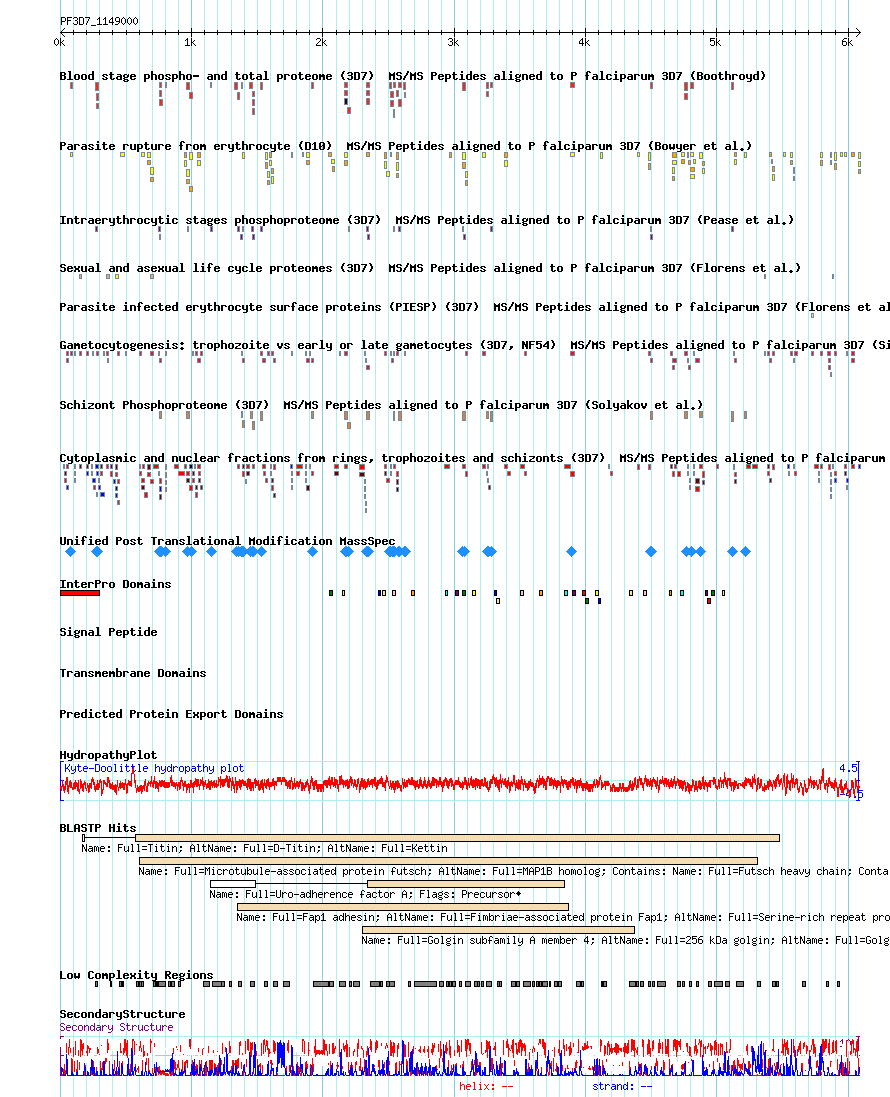
\includegraphics[width=7cm]{figs/plasmodbview}
\caption{\str{PlasmoDB Structural information for PF3D7\_1149000} | This includes, amongst others, InterPro domains, secondary structure prediction and export domains. Note that the protein product of PF3D7\_1149000 has been shown to be exported.}
\label{fig:plasmodb}
\end{figure}

The \pf genome and other associated data are already available from several online databases, including the dedicated PlasmoDB (\url{http://plasmodb.org/}) \cite{Aurrecoechea2009} which provides functional genomic data for genes found in several \bn{Plasmodium} species and includes annotations such as gene location, polymorphisms and expression data, as well as some limited structural annotations (Figure 1). No database presently provides a broad range of structural annotations required for construct design, or allows the user to look only at proteins known to be exported to the red blood cell.

% Flexibility and modularity

The software tools available to 



\subsection{Automating Sequence Submission}


\subsection{Collating output formats}


\subsection{Visualisation}


\section{Limitations and Further Work}

%300 words
%------------------------------------------------
\phantomsection
\section*{Acknowledgments}

I am grateful to John Vakonakis for his insight and encouragement whilst supervising this project.

\addcontentsline{toc}{section}{Acknowledgments} % Adds this section to the table of contents

%----------------------------------------------------------------------------------------
%	REFERENCE LIST
%----------------------------------------------------------------------------------------
\phantomsection
\bibliographystyle{unsrt}
\bibliography{references}

%----------------------------------------------------------------------------------------

\end{document}